\section{Introduction}

Distributed-memory systems are generally used for large-scale
simulations. To program such systems, Message Passing Interface (MPI) is
widely adopted. However, programming with MPI is difficult because
programmers must describe inter-process communications with
consideration of the execution flow of their programs, which might cause
deadlocks or wrong results.

To address this issue, a parallel language named High Performance
Fortran (HPF) was proposed in 1991. With HPF, programmers can execute their
serial programs in parallel by inserting minimal directives into
them. If the programmers specify data distribution with HPF directives,
the compilers do all other tasks for parallelization (e.g. communication
generation and work distribution). However, HPF was not widely accepted
eventually because the compilers' automatic processing prevents the
programmers from performance tuning, and the performance depends heavily
on the environment (e.g. compiler and hardware)

\begin{mynote}
  For more detail, please refer: Ken Kennedy, Charles Koelbel and Hans
  Zima: The Rise and Fall of High Performance Fortran: An Historical
  Object Lesson, Proc. 3rd ACM SIGPLAN History of Programming Languages
  Conf. (HOPL-III), pp.~7-1-7-22 (2007).
\end{mynote}

In such circumstance, to develop a new parallel programming model that
enables easy parallelization of existing serial programs and design a
new language based on it, ``the XMP Specification Working Group'' was
established in 2008. This group utilized the lessons from the experience
of HPF to define a new parallel language {\it XcalableMP (XMP)}. The
group was reorganized to one of the working groups of PC Cluster
Consortium in 2011.

It is learned from the lessons of HPF that more automatic processing of
compilers increases the gap between a program and its execution, and, as
a result, decreases the usability of the language.
%
In XMP, the programmers specify explicitly the details of parallel
programs on the basis of compiler directives to make their execution
easy-to-understand. In particular, they can specify explicitly
communication, synchronization, data mapping, and work mapping
to facilitate performance tuning. In addition, XMP supports features for
one-sided communication on each process, which was not available in
HPF. This feature might enable programmers to implement parallel
algorithms more easily.

In this chapter, an overview of the programming model and language
specification of XMP is shown. You can find the latest and complete
language specification of XMP in: XcalableMP Specification Working
Group, XcalableMP Specification Version 1.4,
\url{http://xcalablemp.org/download/spec/xmp-spec-1.4.pdf} (2018).


%%%%%%%%%%%%%%%%%%%%%%%%%%%%%%%%%%%%%%%%%%%%%%%%%%%%%%%%%%%%%%%%%%%%%
\subsection{Target Hardware}

The target of {\XMP} is distributed-memory multicomputers
(Fig.~\ref{fig1}). Each compute node, which may contain several
cores, has
its own local memory (shared by the cores, if any), and is connected
with the others via an interconnection network.
%
Each node can access its local memory directly and remote memory (the
memory of another node) indirectly (i.e. via inter-node 
communication). However, it is assumed that accessing remote memory may
be much slower than accessing local memory.

\begin{figure}
  \centering
  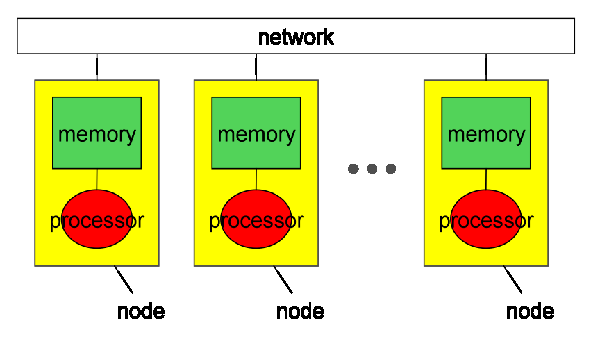
\includegraphics[width=10cm]{figs/Fig1.eps}
  \caption{Target hardware of XMP.}\label{fig1}
\end{figure}


%%%%%%%%%%%%%%%%%%%%%%%%%%%%%%%%%%%%%%%%%%%%%%%%%%%%%%%%%%%%%%%%%%%%%
\subsection{Execution Model}

The execution entities in an XMP program are referred to as XMP {\nodes}
or, more simply, {\nodes}, which has its own memory and can communicate
with each other.

An {\XMP} program execution is based on the Single Program Multiple Data
(SPMD) model, where each {\node} starts execution from the same main
routine, and continues to execute the same code independently
(i.e. asynchronously) until it encounters an {\XMP} construct
(Fig.~\ref{fig:exec_model}).

A set of {\nodes} that executes a procedure, statement, loop,
a block, etc. is referred to as its {\it \Term{executing node set}}, and
is determined by the innermost {\tt task}, {\tt loop}, or {\tt array}
directive surrounding it dynamically, or at runtime.
%
The {\it \Term{current executing node set}} is an {\bf executing node set} of
the current context, which is managed by the {\XMP} runtime system on
each {\node}.

The {\bf current executing node set} at the beginning of the program
execution, or {\it \Term{entire node set}}, is a {\nset} that
contains all the available {\nodes}, which can be specified in an 
implementation-defined way (e.g. through a command-line option).

When a {\node} encounters at runtime either a {\tt loop}, {\tt array}, or
{\tt task} construct, and is contained by the {\nset} specified
(explicitly or implicitly) by the {\tt on} clause of the directive, it
updates the {\bf current executing node set} with the specified one and
executes the body of the construct, after which it resumes the last
{\bf executing node set} and proceeds to execute the subsequent statements.

In particular, when a {\node} in the {\bf current executing node set} encounters a
{\tt loop} or an {\tt array} construct, it executes the loop or the array
assignment in parallel with the other {\nodes}, so that each iteration of the
loop or element of the assignment is independently executed by the {\node}
in which the specified data element resides.

When a {\node} encounters a synchronization or a communication directive,
synchronization or communication occurs between it and the other {\nodes}.
%
That is, such {\it \Term{global constructs}} are performed collectively
by the {\bf current executing nodes}.
%
Note that neither synchronization nor communication occurs unless these
constructs are specified.

\begin{figure}
  \centering
  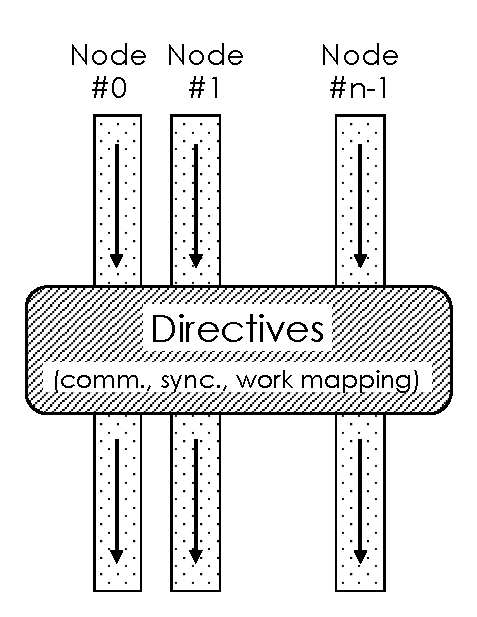
\includegraphics[width=4.5cm]{figs/execution.eps}
  \caption{Execution model of XMP.}\label{fig:exec_model}
\end{figure}


%%%%%%%%%%%%%%%%%%%%%%%%%%%%%%%%%%%%%%%%%%%%%%%%%%%%%%%%%%%%%%%%%%%%%
\subsection{Data Model}

There are two classes of data in {\XMP}: {\it \Term{global data}} and
{\it \Term{local data}}. Data declared in an {\XMP} program are {\local} by
default.

{\bf Global data} are distributed onto a {\nset} by
the {\tt align} directive (see section \ref{sub:align}). Each fragment
of distributed {\bf global data} is allocated in the local memory of a {\node} in the
{\nset}.

{\bf Local data} comprises all data that are not {\bf global}. They are replicated
within the local memory of each of the {\bf executing nodes}.

A {\node} can access directly only local data and sections of {\bf global data}
that reside in its local memory.
%
To access data in remote memory, explicit communication must be
specified in such ways as global communication constructs and
{\coarray} assignments.

% In particular, in {\XMPF}, for common blocks that include any global
% variables, it is implementation-defined what storage sequences they
% occupy and how storage association is defined between two of them.

\begin{figure}
  \centering
  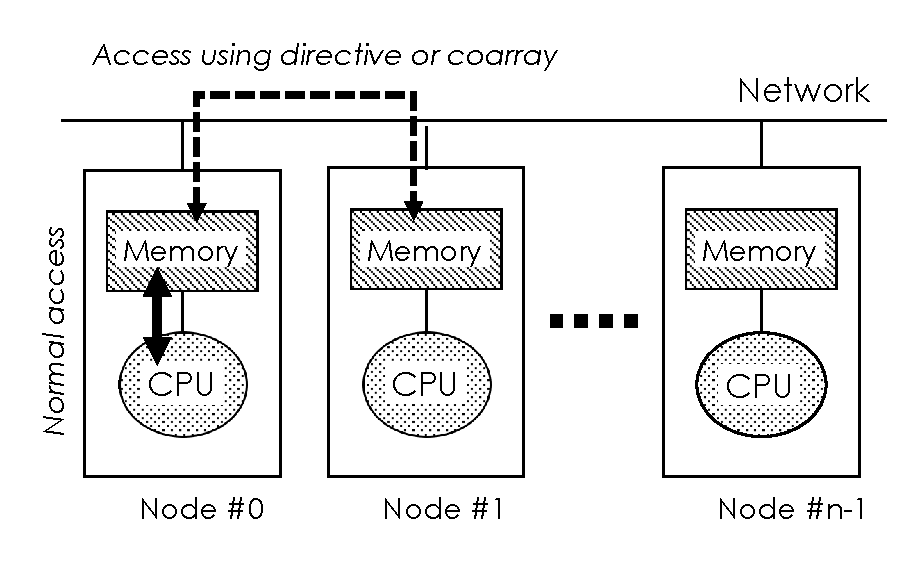
\includegraphics[width=10cm]{figs/architecture.eps}
  \caption{Data model of XMP.}\label{fig:data_model}
\end{figure}


%%%%%%%%%%%%%%%%%%%%%%%%%%%%%%%%%%%%%%%%%%%%%%%%%%%%%%%%%%%%%%%%%%%%%
\subsection{Programming Models}

\subsubsection{Partitioned Global Address Space}

XMP can be classified as a {\it partitioned global address space (PGAS)}
language, such as Co-Array Fortran~\cite{caf}, Unified Parallel
C~\cite{upc}, and Chapel~\cite{chapel}.

In such PGAS languages, multiple executing entities (i.e. threads, processes,
or {\nodes} in XMP) share a part of their address space, which is, however,
partitioned and a portion of which is local to each executing entity.

The two programming models, global-view and local-view, that XMP
supports to achive high performance and productivity on PGAS are
explained below.

\subsubsection{Global-view Programming Model}

The global-view programming model is useful when, starting from a
serial version of a program, the programmer parallelizes it in a
data-parallel style by adding directives with minimum modification.
%
Based on this model, the programmer specifies the distribution of data among
{nodes} using the data distribution directives.
%
The {\tt loop} construct assigns each iteration of a loop to the {\node}
at which the computed data is located. 
%
The global-view communication directives are used to synchronize {\nodes},
maintain the consistency of shadow areas of distributed data, and move
sections of distributed data globally.
%
Note that the programmer must specify explicitly communication to make
all data references in their program local using appropriate
directives.

In many cases, the {\XMP} program following to the global-view
programming model is based on a serial program, and it can produce
the same result, regardless of the number of {\nodes} (Fig.~\ref{fig2}).

There are three groups of directives for this model:

\begin{itemize}
  \item {\it Data mapping,} which specifies the data distribution and mapping
		to {\nodes}
  \item {\it Work mapping (parallelization),} which specifies the work
		distribution and mapping to {\nodes}.
		% The {\tt loop} construct maps
		% each iteration of a loop to nodes owning specific data
		% elements. The {\tt task} construct defines a set amount of work
		% as a {\it \Term{task}}, and assigns it to a specific node set.
  \item {\it Communication and synchronization,} which specify how a
		{\node} communicates and synchronizes with the other {\nodes}.
		% In
		% {\XMP}, inter-node communication must be explicitly specified by
		% the programmer. The compiler guarantees that no communication
		% occurs unless it is explicitly specified by the programmer.
\end{itemize}

Because these
directives are ignored as a comment by the 
compilers of base languages ({\Fort} and {\C}), an {\XMP} program can
usually be compiled by them to ensure that they run properly.

\begin{figure}
  \centering
  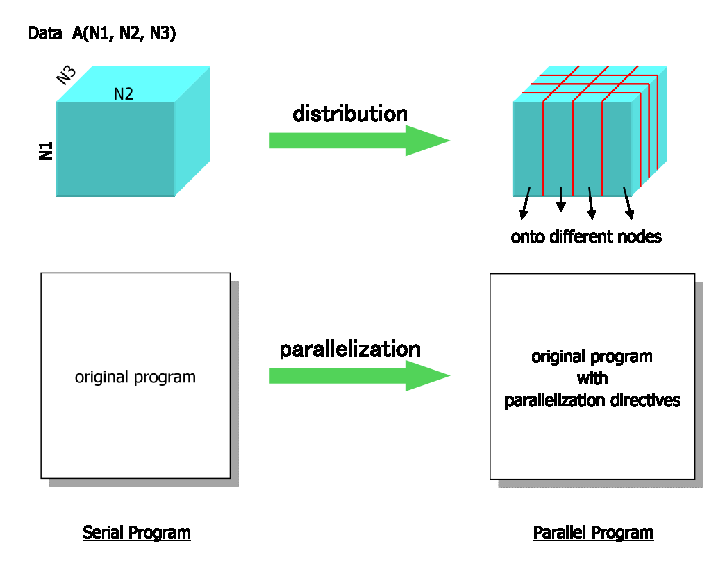
\includegraphics[width=10cm]{figs/Fig2.eps}
  \caption{Parallelization based on the global-view programming model.}
\label{fig2}
\end{figure}


\subsubsection{Local-view Programming Model}

The local-view programming model is suitable for programs that
implement an algorithm and a remote data reference that are to
be executed by each {\node} (Fig.~\ref{fig3}).

For this model, some language extensions and 
directives are provided. The {\coarray} notation, which is imported from
{\Fort} 2008,
is one such extension, and can be used to explicitly specify data on which {\node}
is to be accessed. For example, the expression of {\tt
A(i)[N]} is used to access an array element of {\tt A(i)} located on the
{\node} {\tt N}.
%
If the access is a reference, then a one-sided communication to read the
value from the remote memory (i.e. the {\it get} operation) is issued
by the {\bf executing node}.
If the access is a definition, then a one-sided communication to write
the value to the remote memory (i.e. the {\it put} operation) is issued by
the {\bf executing node}.

\begin{figure}
  \centering
  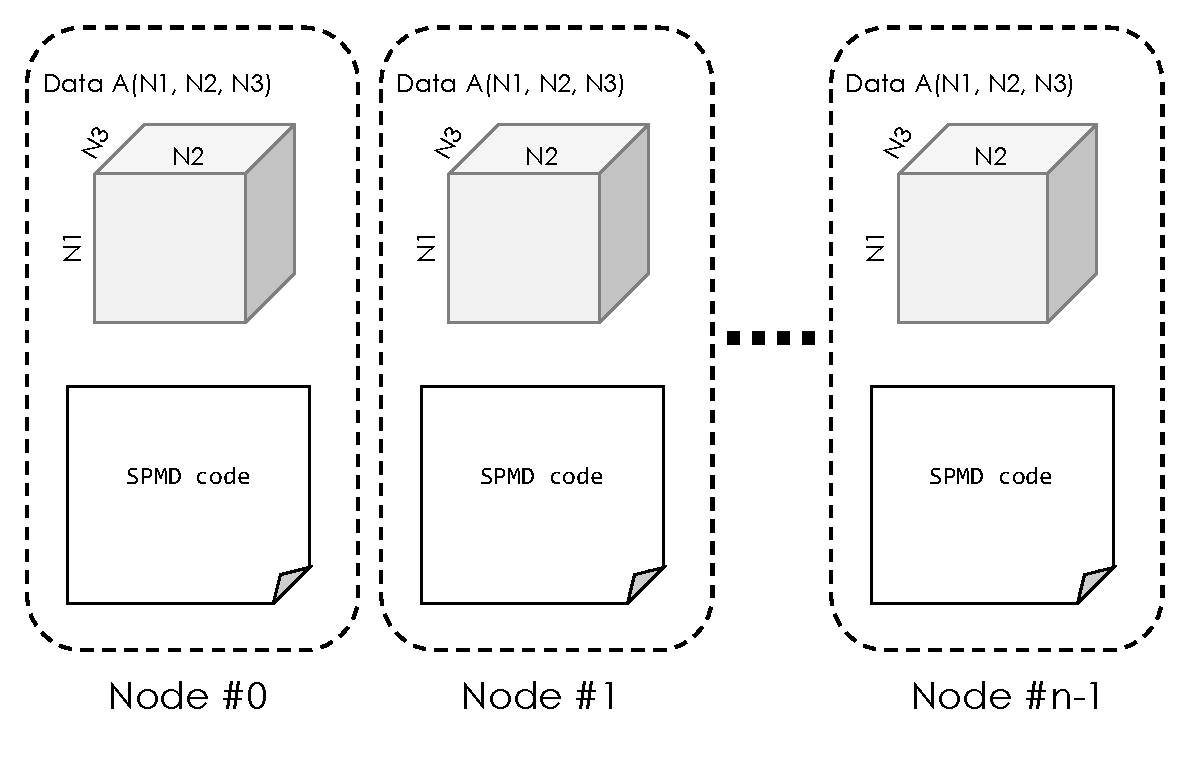
\includegraphics[width=10cm]{figs/Fig3.eps}
  \caption{Local-view programming model.}
\label{fig3}
\end{figure}


\subsubsection{Mixture of Global View and Local View}

In the global-view model, {\nodes} are used to distribute data and works. In the
local-view model, {\nodes} are used to address remote data in the {\coarray}
notation.
%
In application programs,
the programmers should choose an appropriate data model according to the
characteristics of their program. Fig.~\ref{fig4} illustrates the global view
and the local view of data.

Data can have both a global view and a local view, and can be accessed
in both of the views. {\XMP} provides a directive to give the {\local} name
(alias) to {\bf global data} declared in the global-view programming model
to enable them to also be accessed in the local-view programming
model. This feature is useful to optimize a certain part of a program
by using explicit remote data access in the local-view programming
model.

\begin{figure}
  \centering
  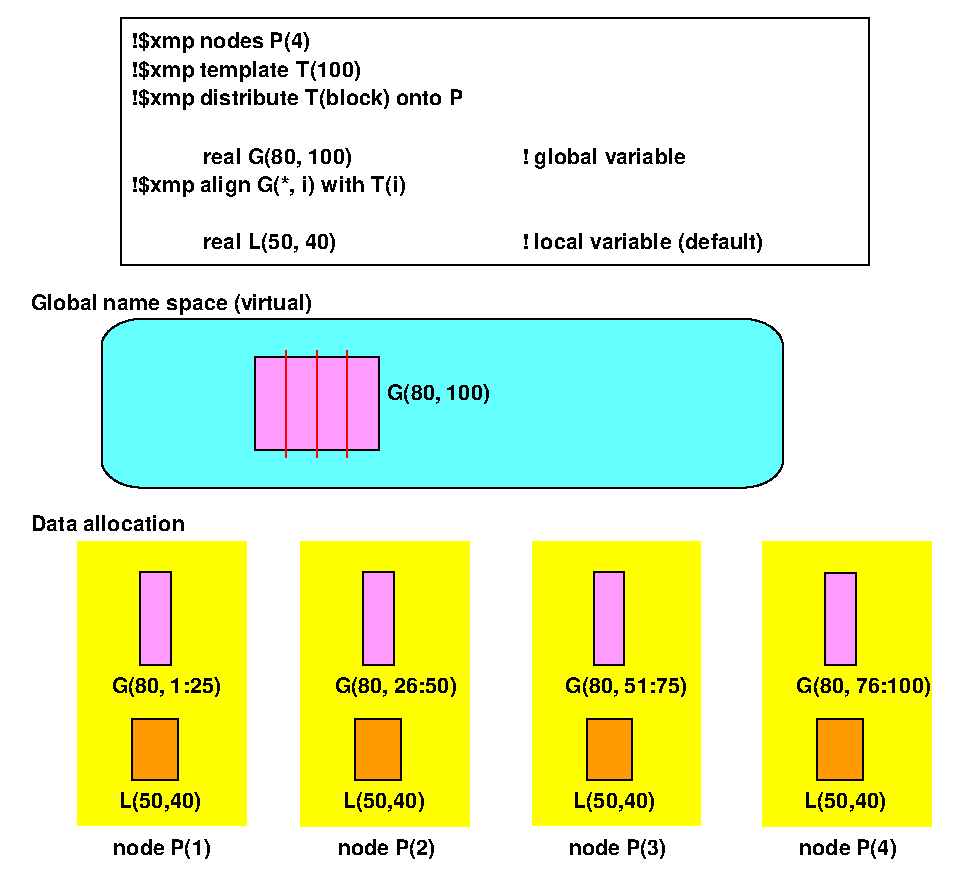
\includegraphics[width=10cm]{figs/Fig4.eps}
  \caption{Global view and local view.}
  \label{fig4}
\end{figure}


\subsection{Base Languages}

The XcalableMP language specification is defined on the basis of Fortran
and C as the base languages. More specifically, the base language of
XcalableMP Fortran is Fortran 90 or later, and that of XcalableMP C is
ISO C90 (ANSI C89) or later with some extensions (see below).

\subsubsection{Array Section in {\XMPC}}

% \label{173437_31Oct14}

% \subsubsection*{Synopsis}

% The array section notation is a notation to describe a part of an array, 
% which is adapted in Fortran.

% \subsubsection*{Syntax}
% \index{array section in XMP/C}
% \index{Syntax!array section in XMP/C}

% \begin{tabular}{llll}
% \verb![C]! & {\it array-section} & {\bf is} & {\it array-name}{\tt [} \{
%  {\it triplet} $\vert$ {\it int-expr} \} {\tt ]}...
% \end{tabular}

% \vspace{0.5cm}

% %where {\it triplet} must be one of:
% where {\it triplet} is:

% \vspace{0.3cm}

% \begin{tabular}{ll}
%  \hspace{0.5cm} & {\openb}{\it base}{\closeb} {\tt :}
%   {\openb}{\it length}{\closeb} {\openb}{\tt :} {\it step}{\closeb}\\
% % \hspace{0.5cm} & {\tt :} \\
% \end{tabular}

% \subsubsection*{Description}

In {\XMPC}, the base language C is extended so that a part of an array,
that is, an {\it array section} or {\it subarray}, can be put in an {\it
array assignment statement}, which is described in \ref{subsubsec:Array
assignment statements in C}, and some {\XMP} constructs.
%
An array section is built from a subset of the elements of an array,
which is specified by a sequence of square-bracketed integer expressions
or {\it triplets}, which are in the form of:

\begin{center}
  [ {\it base} ] {\tt :} [ {\it length} ] [ {\tt :} {\it step} ]
\end{center}

When {\it step} is positive, the {\it triplet} specifies a set of
subscripts that is a regularly spaced integer sequence of length {\it
length} beginning with {\it base} and proceeding in increments of {\it
step} up to the largest.
%
The same applies to negative {\it step} too.

When {\it base} is omitted, it is assumed to be 0. When {\it length}
is omitted, it is assumed to be the number of remainder elements of the
dimension of the array. When {\it step} is omitted, it is assumed to be 1.

% \subsubsection*{Example}
% \index{Example!array section in XMP/C}

Assuming that an array {\tt A} is declared by the following statement,

\vspace{0.3cm}

\begin{tabular}{ll}
\hspace{0.5cm} & {\tt int A[100];} \\
\end{tabular}

\vspace{0.3cm}

\noindent some array sections can be specified as follows:

\vspace{0.3cm}

\begin{tabular}{lll}
\hspace{0.5cm} & {\tt A[10:10]} & array section of 10 elements from {\tt
 A[10]} to {\tt A[19]} \\
 & {\tt A[10:]} & array section of 90 elements from
		  {\tt A[10]} to {\tt A[99]}\\
 & {\tt A[:10]} & array section of 10 elements from {\tt A[0]} to {\tt
	 A[9]} \\
 & {\tt A[10:5:2]} & array section of 5 elements from {\tt A[10]} to
	 {\tt A[18]} by step 2 \\
 & {\tt A[:]}      & array section of the whole of {\tt A} \\
\end{tabular}


\subsubsection{Array Assignment Statement in {\XMPC}}
\label{subsubsec:Array assignment statements in C}

% \subsubsection*{Synopsis}

% An array assignment statement copies a value into each element of
% an array section.

% \subsubsection*{Syntax}
% \index{array assignment in XMP/C}
% \index{Syntax!array assignment in XMP/C}

% \begin{tabular}{ll}
% \verb![C]! & {\it array-section} {\openb}{\tt :}{\tt [}{\it int-expr}{\tt
%  ]}...{\closeb} {\tt =} {\it expression}{\tt ;}\\
% \end{tabular}

% \subsubsection*{Description}

In {\XMPC}, the base language C is also extended so that it supports
array assignment statements just as Fortran does.

With such statement, the value of each element of the result of the
right-hand side expression is assigned to the corresponding element of
the array section on the left-hand side.
%
When an operator or an elemental function
%(see section \ref{094142_25Sep13})
is applied to array sections in the right-hand side
expression, it is evaluated to an array section that has the same shape
as that of the operands or arguments, and each element of which is the
result of the operator or function applied to the corresponding element
of the operands or arguments. A scalar object is assumed to be an array
section that has the same shape as that of the other array section(s) in
the expression or on the left-hand side, and
where each element has its value.

Note that an array assignment is a statement, and therefore cannot
appear as an expression in any other statements.

% \subsubsection*{Restrictions}

% \begin{itemize}
%  \item \verb![C]! any array section appearing in the right-hand side expression and
% 	   the left-hand side must have the same shape, i.e., the same number of
% 	   dimensions and size of each dimension.
%  % \item \verb![C]! When the right-hand side is an array section, the left-hand side and the right-hand side
%  %       must have the same shape, i.e., the same number of dimensions and
%  %       size of each dimension.
%  \item \verb![C]! If {\it array-section} on the left-hand side is followed by
%        ``{\tt :}{\tt [}{\it int-expr}{\tt ]}...'', it must be a coarray.
%  % \item \verb![C]! If {\it variable} on the right-hand side is followed by
%  %       ``{\tt :}{\tt [}{\it int-expr}{\tt ]}...'', it must be a coarray.
% \end{itemize}

% \subsubsection*{Examples}
% \index{Example!array assignment in XMP/C}

An array assignment statement in the fourth line copies the five elements
from {\tt B[0]} to {\tt B[4]} into the elements from {\tt A[5]} to {\tt
A[9]}.

\hspace{\hsize}
\begin{XCexample}
int A[10];
int B[5];
    ...
A[5:5] = B[0:5]; 
\end{XCexample}


% \subsubsection{Built-in Functions for Array Section}
% \index{built-in functions of XMP/C}

% Some built-in functions are defined that can accept one or more array
% sections as arguments. In addition, some of them are array-valued.
% %
% Such array-valued functions can appear in the right-hand side of an
% array assignment statement, and should be preceded by the {\tt array}
% directive if the array section is distributed.

% All of the built-in functions for array sections are described in
% Sections \ref{094142_25Sep13} and \ref{112125_19Sep13}.


% \subsubsection{Pointer to Global Data}
% \label{sec:pointer to global data}

% \paragraph{Name of Global Array}

% The name of a global array is considered to represent an abstract entity
% in the {\XMP} language. It is not interpreted as the pointer to the array,
% while the name of a local array is.

% However, the name of a global array that appears in an expression is
% evaluated to the base address of its local section on each node. The
% pointer can be operated on each node as if it were a normal (local)
% pointer.

% \paragraph{Address-of Operator}
% \index{address-of operator}

% The result of the address-of operator (``{\tt \&}'') applied to an
% element of a global array is the pointer to the corresponding element of
% its local section. Note that the value of the result pointer is defined
% only on the node that owns the element. The pointer can be operated on
% the node as if it were a normal (local) pointer.

% As a result, for a global array {\tt a}, {\tt a} and {\tt \&a[0]} are
% not always evaluated to the same value.

% \subsubsection{Support for Intrinsic/Built-in Functions of the Base
% 	  Languages}

% This section describes how intrinsic/built-in functions of the base
% languges work on XMP's global arrays.

% Many other intrinsic and library procedures, such as mapping inquiry
% functions and transformational procedures, are defined in XMP. See the
% language specification for their detail.

% \paragraph{Array Intrinsic Functions in {\XMPF}}
% \index{array intrinsic functions}

% The array intrinsic functions of the base language Fortran are
% classified into three classes: {\it inquiry}, {\it elemental}, and
% {\it transformational}.

% It is specified as follows how these functions work in the XMP/F
% programs when a global array appears as an argument.

% \begin{itemize}
%  \item Inquiry functions

%        The inquiry functions with a global array or its subobject
%        being an argument are regarded as inquiries about the global
%        array, and return its ``global'' properties as if it were not
%        distributed.

%  \item Elemental functions

%        The result of the elemental functions with a global array or
%        its subobject being an argument has the same shape and
%        mapping as the argument.
% %
%        Note that such a reference of these elemental functions is in
%        effect limited to be in the {\tt array} construct.

%  \item Transformational functions

%        It is unspecified how the transformational functions work when a
%        global array or its subobject appears as an argument.
% %
%        A processor shall detect such a reference of these functions
%        and issue a warning message for it.
% %
%        Some intrinsic transformational subroutines are defined in
%        section \ref{112125_19Sep13} as alternatives to these
%        transformational functions.

% \end{itemize}


% \paragraph{Built-in Elemental Functions in {\XMPC}}
% \label{094142_25Sep13}
% \index{built-in elemental functions}

% Some built-in elemental functions that can operate each element of
% array arguments are defined in {\XMPC}. Such a built-in function
% accepts one or more array sections as its arguments and returns an
% array-valued result having the same shape and mapping as the argument.
% %
% The values of the elements of the result are the same as what would have
% been obtained if the scalar function of the C standard library had
% been applied separately to the corresponding elements of each array
% argument.

% These functions may appear on the right-hand side of an array
% assignment statement, and it should be preceded by the {\tt array}
% directive if the array section is distributed.

% Table \ref{tab:elemental_c} shows the list of built-in elemental
% functions in {\XMPC}. Their elementwise behavior is the same as those of
% the corresponding functions in the C standard library.

% \begin{table}[h]
%  \caption[Built-in elemental functions in {\XMPC}]{Built-in elemental
%  functions in {\XMPC}. (The first line refers to the element type of their
%  argument(s) and return value.)}
%  \label{tab:elemental_c}
%  \begin{center}
%  \begin{tabular}{c|c|c} \hline\hline
%  double & float & long double \\ \hline
%  acos & acosf & acosl \\
%  asin & asinf & asinl \\
%  atan & atanf & atanl \\
%  atan2 & atan2f & atan2l \\
%  cos & cosf & cosl \\
%  sin & sinf & sinl \\
%  tan & tanf & tanl \\

% % acosh & acoshf & acoshl \\
% % asinh & asinhf & asinhl \\
% % atanh & atanhf & atanhl \\
%  cosh & coshf & coshl \\
%  sinh & sinhf & sinhl \\
%  tanh & tanhf & tanhl \\

%  exp & expf & expl \\
% % exp2 & exp2f & exp2l \\
% % expm1 & expm1f & expm1l \\
%  frexp & frexpf & frexpl \\
% % ilogb & ilogbf & ilogbl \\
%  ldexp & ldexpf & ldexpl \\
%  log & logf & logl \\
%  log10 & log10f & log10l \\
% % log1p & log1pf & log1pl \\
% % log2 & log2f & log2l \\
% % logb & logbf & logbl \\
% %% modf & modff & modfl \\
% % scalbn & scalbnf & scalbnl \\
% % scalbln & scalblnf & scalblnl \\

% % cbrt & cbrtf & cbrtl \\
%  fabs & fabsf & fabsl \\
% % hypot & hypotf & hypotl \\
%  pow & powf & powl \\
%  sqrt & sqrtf & sqrtl \\

% % erf & erff & erfl \\
% % erfc & erfcf & erfcl \\
% % lgamma & lgammaf & lgammal \\
% % tgamma & tgammaf & tgammal \\

%  ceil & ceilf & ceill \\
%  floor & floorf & floorl \\
% % near byint near byintf near byintl \\
% % rint & rintf & rintl \\
% % lrint & lrintf & lrintl \\
% % llrint & llrintf & llrintl \\
% % round & roundf & roundl \\
% % lround & lroundf & lroundl \\
% % llround & llroundf & llroundl \\
% % trunc & truncf & truncl \

%  fmod & fmodf & fmodl \\ \hline
% % remainder & remainderf & remainderl \\
% % remquo & remquof & remquol \\
% %
% % copysign & copysignf & copysignl \\
% % nan & nanf & nanl \\
% % next after next afterf next afterl \\
% % next toward next towardf & next towardl \\
% %
% % fdim & fdimf & fdiml \\
% % fmax & fmaxf & fmaxl \\
% % fmin & fminf & fminl \\

% % fma & fmaf & fmal \\
%  \end{tabular} 
%  \end{center}
% \end{table}


%%%%%%%%%%%%%%%%%%%%%%%%%%%%%%%%%%%%%%%%%%%%%%%%%%%%%%%%%%%%%%%%%%%%%
\subsection{Interoperability}

Most of existing parallel applications are written with MPI. It is not
realistic to port them over to XMP because each of them consists of
millions of lines.

Because XMP is interoperable with MPI, users can develop an XMP
application by modifying a part of an existing one instead of rewriting
it totally. Besides, when developing a parallel application from
scratch, it is possible to use XMP to write a complicated part of, for
example, domain decomposition while they use MPI, which could be faster
than XMP, to write a hot-spot part that need to be tuned carefully. In
addition, XMP is interoperable with OpenMP and Python (see Chapter
\ref{python}).

It might be difficult to develop an application with just one
programming language or framework since it generally has its own strong
and weak points. Thus, an XMP program is interoperable with those in
other languages to provide both high productivity and performance.